% -*- LaTeX -*-
% -*- coding: utf-8 -*-
%
% michael a.g. aïvázis <michael.aivazis@para-sim.com>
% (c) 2003-2017 all rights reserved
%

\section{case study}
\subsection{description}

\begin{frame}
  \frametitle{Case study: assembling a digital elevation model}
%
  % \vskip -5ex
%
  \begin{columns}[c]
    \begin{column}{.4\textwidth}
      \only<1>{
        \begin{center}
          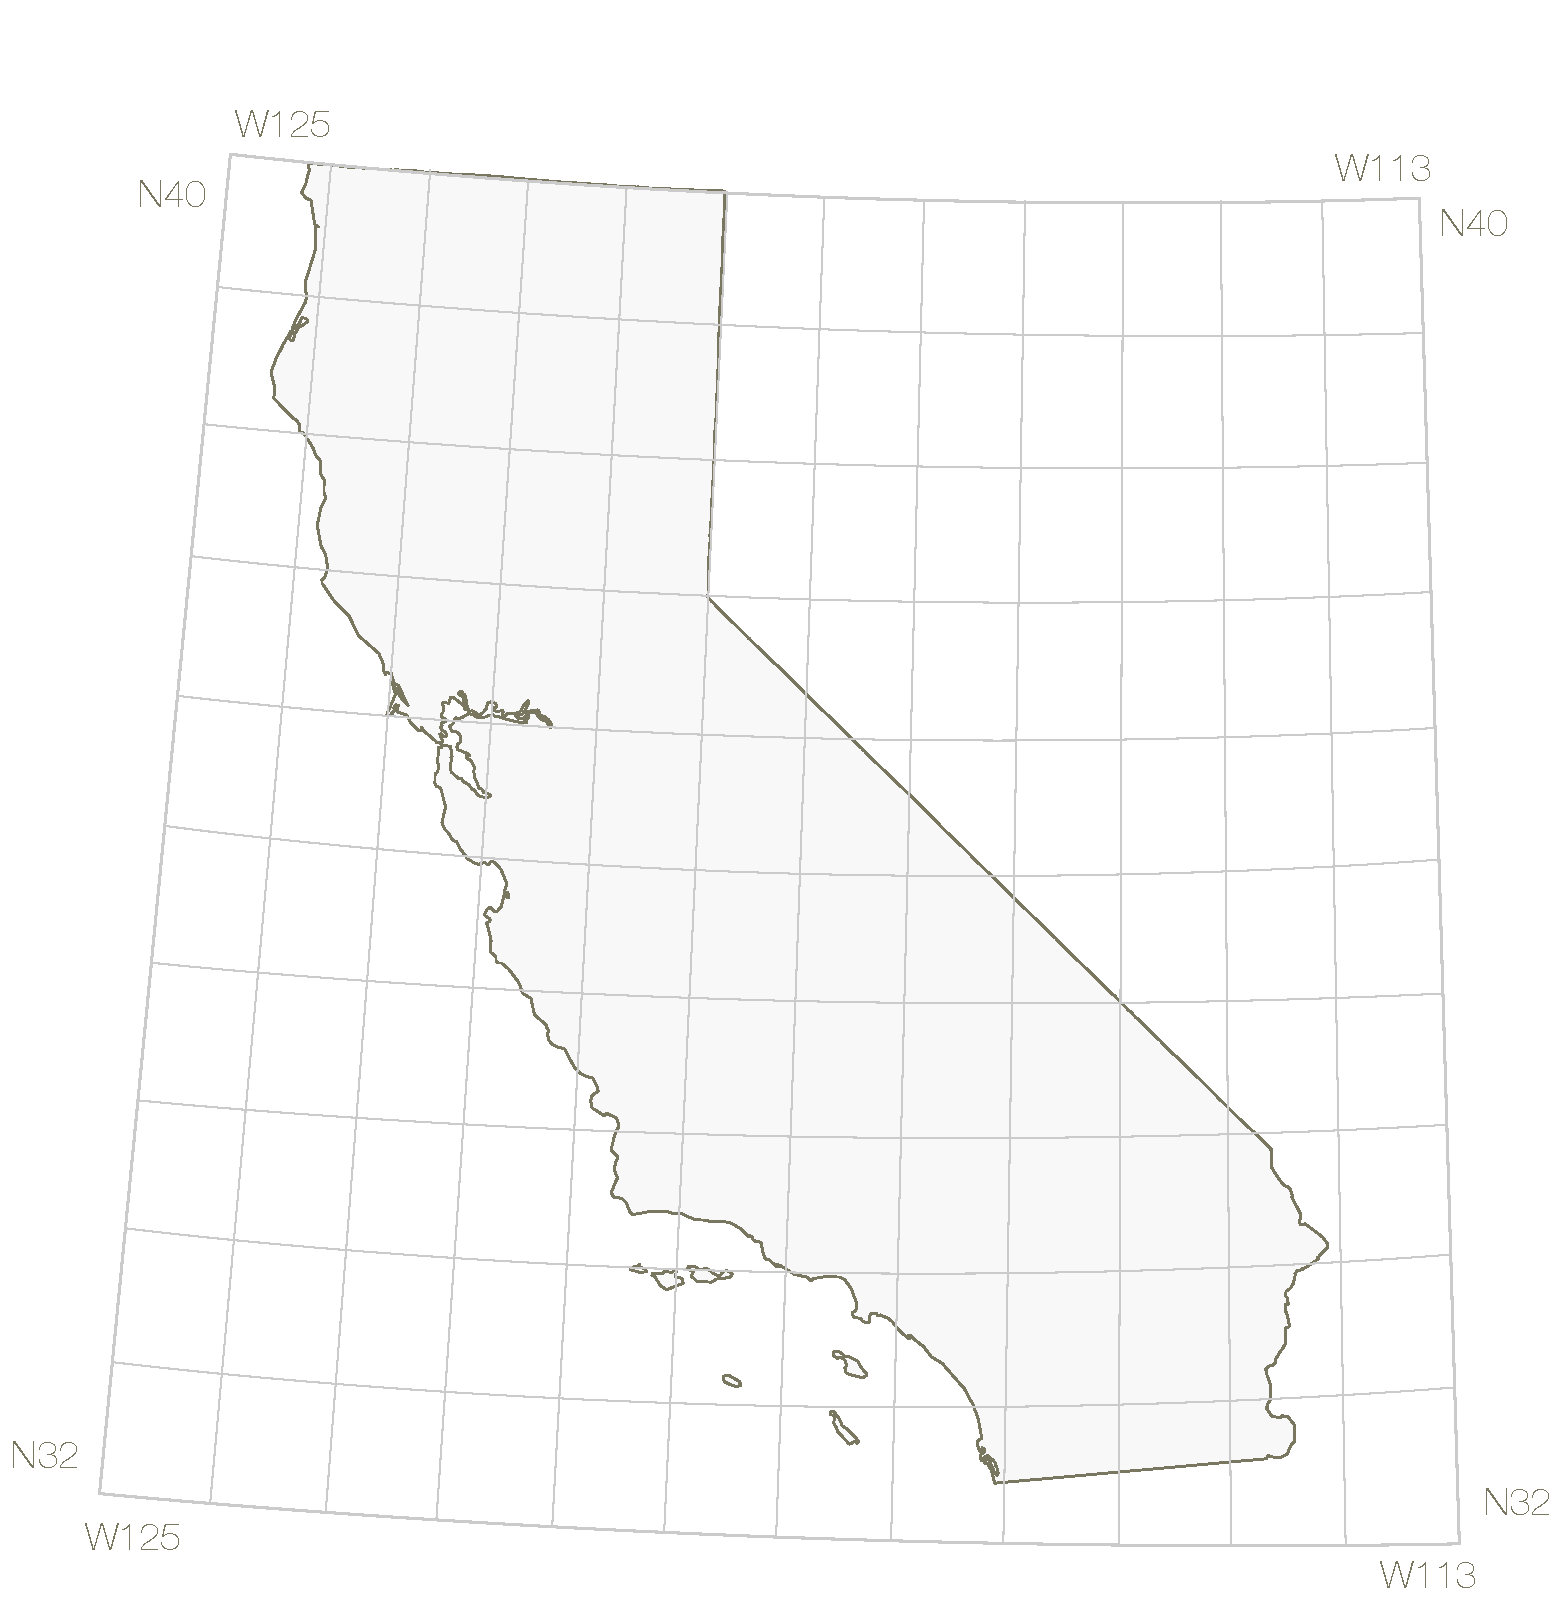
\includegraphics[width=.95\textwidth]{dem-california}
        \end{center}
      }
      \only<2>{
        \begin{center}
          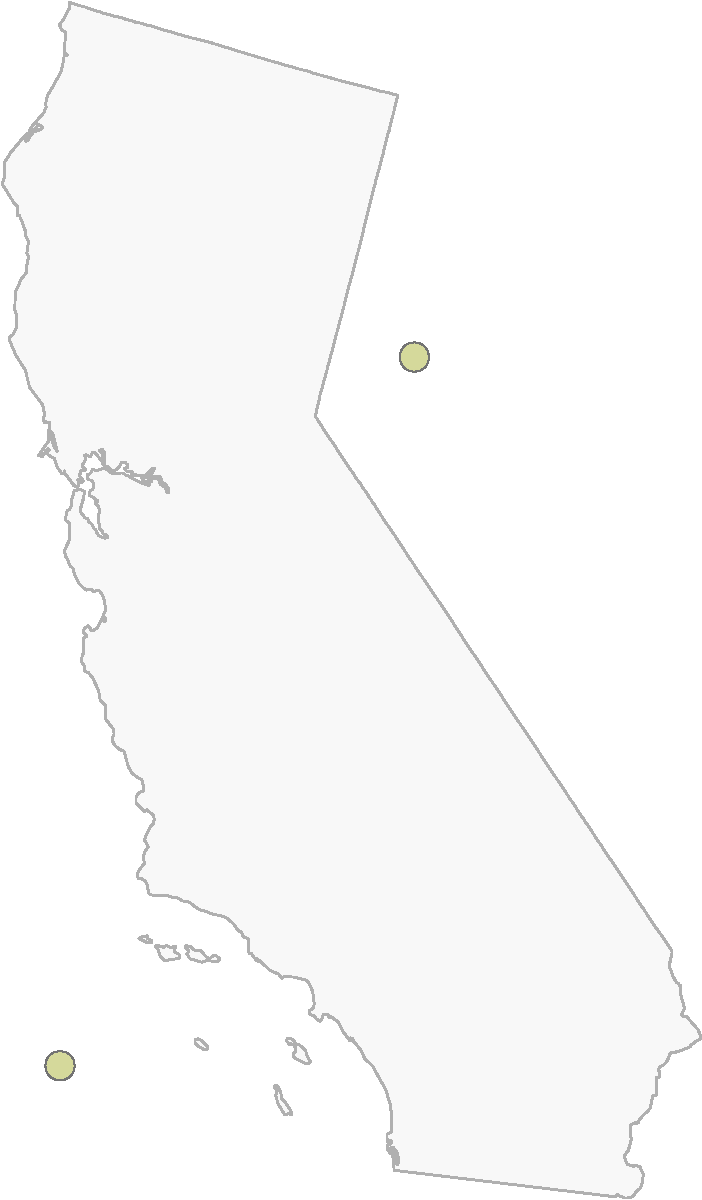
\includegraphics[width=.95\textwidth]{dem-region}
        \end{center}
      }
      \only<3>{
        \begin{center}
          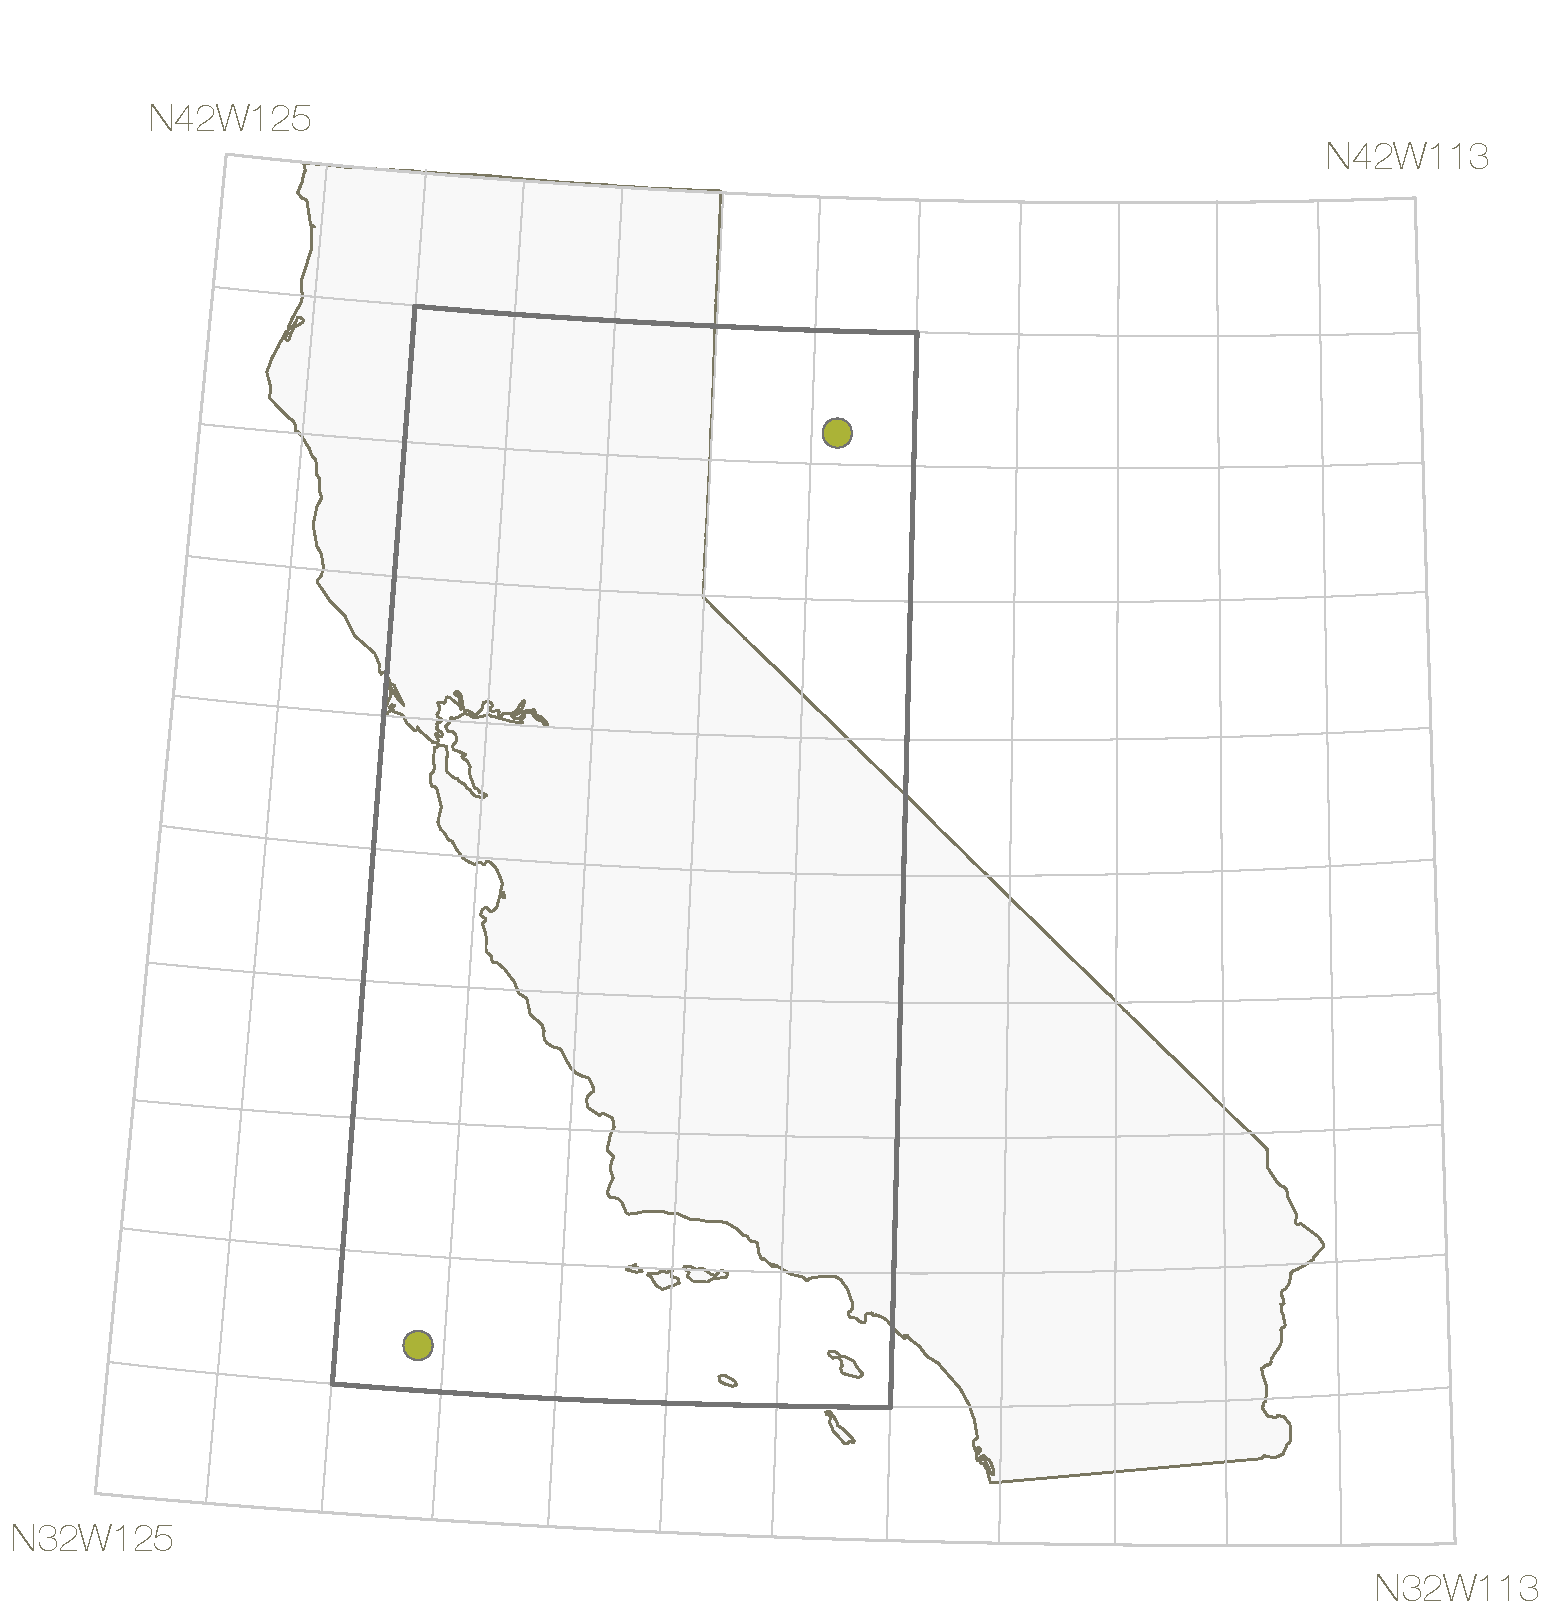
\includegraphics[width=.95\textwidth]{dem-bbox}
        \end{center}
      }
      \only<4->{
        \begin{center}
          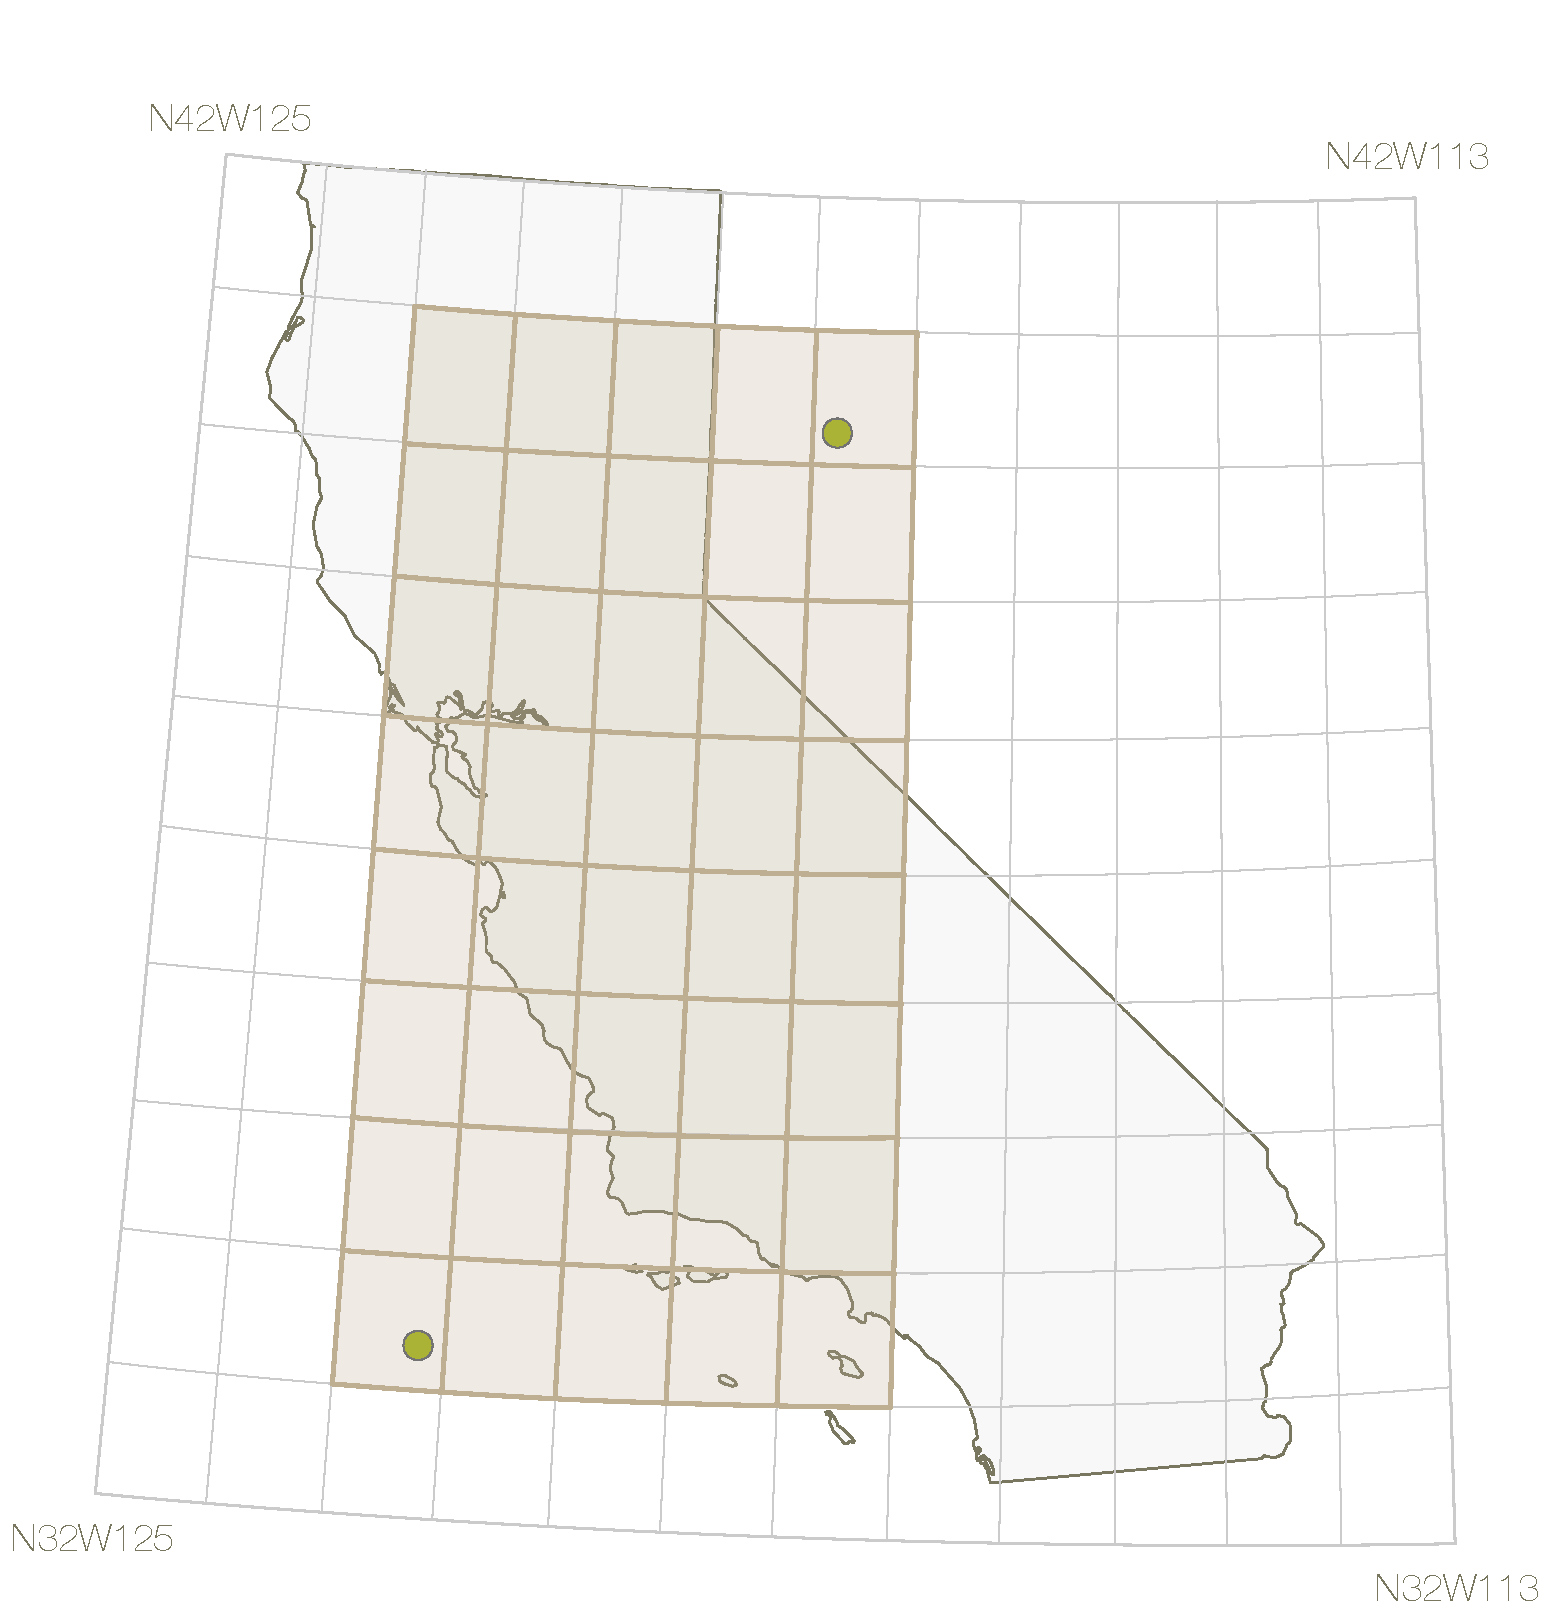
\includegraphics[width=.95\textwidth]{dem-tiles}
        \end{center}
      }
    \end{column}
    %
    \begin{column}{.5\textwidth}
      \begin{itemize}
      \item<1-> Given a region of the planet
      \item<2-> pick a few points
      \item<3-> compute their bounding box
      \item<4-> tile the box
      \item<5-> stitch the digital elevation model
      \end{itemize}
    \end{column}
    %
  \end{columns}
%
\end{frame}

%-----------------------------------
\subsection{outline}

\begin{frame}
%
  \frametitle{Outline of the implementation}
%
%
  \begin{itemize}
%
  \item
%
  \end{itemize}
%
\end{frame}


%%% Local Variables:
%%% mode: latex
%%% TeX-master: "../pyre"
%%% End:

% end of file
